\FloatBarrier
\begin{figure}[!h]
\centering
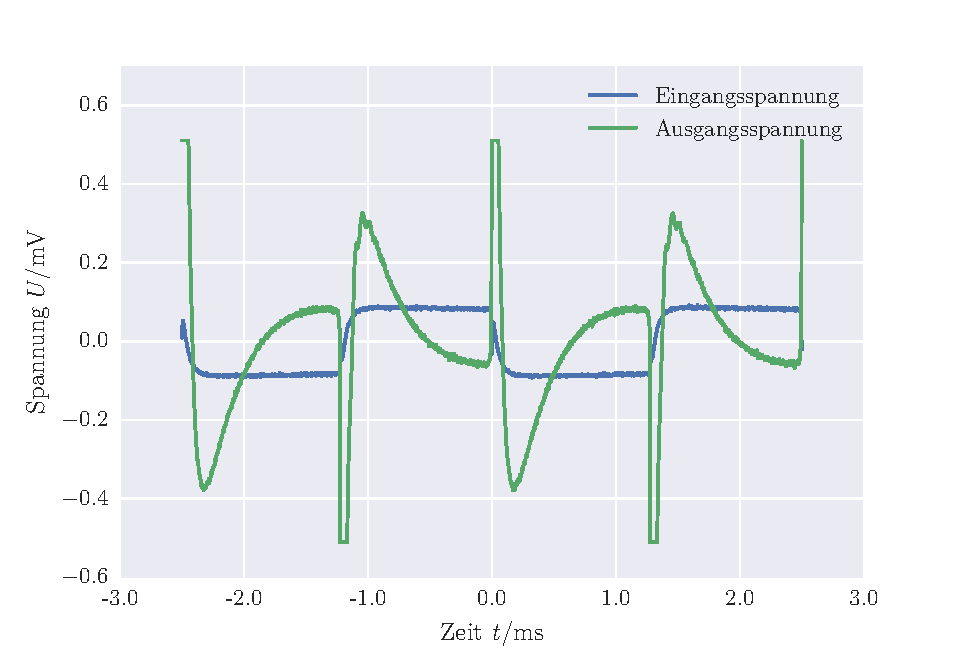
\includegraphics[scale=0.75]{../Grafiken/Differentiator_Oszilloskop_Rechteck.pdf}
\caption{Vom Oszilloskop aufgenommene Ein- und Ausgangsspannungen der Differentiatorschaltung. Auf dem Eingang
	liegt hier eine Rechteckspannung. Die Ausgangsspannung in Form schmalen hohen Peaks entspricht in etwa dem 
	theoretisch zu erwartendem Verlauf eines Delta-Kamms.\label{fig:differentiator_oszilloskop_rechteck}}
\end{figure}
\FloatBarrier